\documentclass[12pt]{article}
\usepackage{amsmath, amssymb, amsthm}
\usepackage{geometry, enumitem, mdframed}
\usepackage{tikz, pgfplots}
\usepackage{graphicx}
\geometry{margin=1in}

\newtheorem{definition}{Definition}
\newtheorem{theorem}{Theorem}
\newtheorem{example}{Example}
\newmdenv[linecolor=red,linewidth=2pt]{warning}
\newmdenv[linecolor=blue,linewidth=2pt]{keypoint}
\newmdenv[linecolor=green,linewidth=2pt]{insight}

\title{ODE Lesson 7: Non-Unique Solutions - Classic Examples and Warnings}
\author{ODE 1 - Prof. Adi Ditkowski}
\date{}

\begin{document}
\maketitle

\section{When Uniqueness Fails}

\begin{keypoint}
\textbf{Core Principle:} Non-uniqueness occurs when the Lipschitz condition fails. This typically happens at points where $\frac{\partial f}{\partial y}$ is unbounded or discontinuous.
\end{keypoint}

\begin{definition}[Non-Unique Solutions]
An IVP has \textbf{non-unique solutions} if multiple distinct functions satisfy both the differential equation and the initial conditions.
\end{definition}

\section{The Classic Example}

\begin{example}[The Square Root Problem]
Consider the IVP:
$y' = 2\sqrt{|y|}, \quad y(0) = 0$

This has infinitely many solutions:
\begin{itemize}
    \item $y_1(x) \equiv 0$ (trivial solution)
    \item $y_2(x) = \begin{cases}
        0 & \text{if } x \leq c \\
        (x-c)^2 & \text{if } x > c
    \end{cases}$ for any $c \geq 0$
    \item $y_3(x) = \begin{cases}
        -(x-c)^2 & \text{if } x < c \\
        0 & \text{if } x \geq c
    \end{cases}$ for any $c \leq 0$
\end{itemize}
\end{example}

\begin{center}
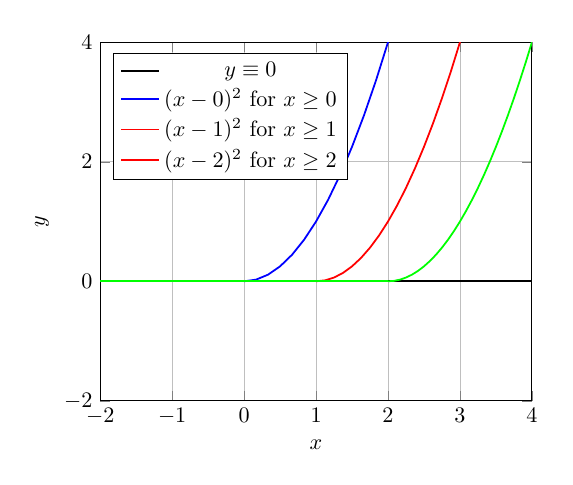
\begin{tikzpicture}[scale=0.8]
\begin{axis}[
    xlabel={$x$},
    ylabel={$y$},
    grid=major,
    xmin=-2, xmax=4,
    ymin=-2, ymax=4,
    legend pos=north west
]
% Trivial solution
\addplot[black, thick] coordinates {(-2,0) (4,0)};
\addlegendentry{$y \equiv 0$}

% Solution starting at x=0
\addplot[blue, thick, domain=0:4] {x^2};
\addlegendentry{$(x-0)^2$ for $x \geq 0$}

% Solution starting at x=1
\addplot[red, thick, domain=-2:1] {0};
\addplot[red, thick, domain=1:4] {(x-1)^2};
\addlegendentry{$(x-1)^2$ for $x \geq 1$}

% Solution starting at x=2
\addplot[green, thick, domain=-2:2] {0};
\addplot[green, thick, domain=2:4] {(x-2)^2};
\addlegendentry{$(x-2)^2$ for $x \geq 2$}
\end{axis}
\end{tikzpicture}
\end{center}

\section{General Pattern for Non-Uniqueness}

\subsection{The Power Law Family}

\begin{theorem}[Power Law Non-Uniqueness]
The IVP $y' = k|y|^\alpha$ with $y(0) = 0$ where $0 < \alpha < 1$ has infinitely many solutions.

General solution family:
$y(x) = \begin{cases}
    0 & \text{if } |x| \leq c \\
    \pm\left[\frac{1-\alpha}{k}(|x|-c)\right]^{\frac{1}{1-\alpha}} & \text{if } |x| > c
\end{cases}$
\end{theorem}

\begin{insight}
\textbf{Geometric Intuition:} The smaller $\alpha$, the "flatter" the slope field near $y = 0$, making it easier for solutions to "peel away" from the $x$-axis.
\end{insight}

\section{Lipschitz Failure Analysis}

\subsection{Why Square Roots Cause Problems}

For $f(y) = |y|^\alpha$ with $0 < \alpha < 1$:
$\frac{\partial f}{\partial y} = \alpha |y|^{\alpha-1} \rightarrow \infty \text{ as } y \rightarrow 0$

\begin{table}[h]
\centering
\begin{tabular}{|c|c|c|c|}
\hline
\textbf{Function} & \textbf{Derivative} & \textbf{Lipschitz at 0?} & \textbf{Unique?} \\
\hline
$y$ & $1$ & Yes & Yes \\
$y^2$ & $2y$ & Yes & Yes \\
$\sqrt{|y|}$ & $\frac{1}{2\sqrt{|y|}}$ & No & No \\
$|y|^{2/3}$ & $\frac{2}{3}|y|^{-1/3}$ & No & No \\
$|y|^{3/2}$ & $\frac{3}{2}|y|^{1/2}$ & Yes & Yes \\
\hline
\end{tabular}
\end{table}

\section{The Peano Phenomenon}

\begin{definition}[Peano Phenomenon]
Solutions that can "branch" - starting from the same initial condition, the solution can follow different paths after some time.
\end{definition}

\begin{example}[Branching Solutions]
Consider the implicit equation: $(y')^2 = 4y$

From $y(0) = 0$, solutions can:
\begin{enumerate}
    \item Stay at $y = 0$ for interval $[0,a]$
    \item Branch upward: $y = (x-a)^2$ for $x \geq a$
    \item Branch downward: $y = -(x-a)^2$ for $x \leq a$
\end{enumerate}
\end{example}

\section{Construction Methods for Non-Unique Solutions}

\subsection{Method 1: Separation of Variables Pitfall}

\begin{warning}
When separating variables in $\frac{dy}{dx} = g(y)h(x)$, if $g(y_0) = 0$, the constant solution $y \equiv y_0$ might be lost!
\end{warning}

\begin{example}[Lost Solutions]
$y' = y(1-y)$
Separating: $\int \frac{dy}{y(1-y)} = \int dx$

This process misses the equilibrium solutions:
\begin{itemize}
    \item $y \equiv 0$
    \item $y \equiv 1$
\end{itemize}
\end{example}

\subsection{Method 2: Clairaut's Equation}

\begin{theorem}[Clairaut's Equation]
Equations of the form $y = xy' + f(y')$ have:
\begin{itemize}
    \item General solution: $y = cx + f(c)$ (family of lines)
    \item Singular solution: The envelope of the family
\end{itemize}
\end{theorem}

\subsection{Method 3: Solution Patching}

\begin{mdframed}[backgroundcolor=yellow!10]
\textbf{Patching Technique:}
If $f(x,y) = 0$ along curve $C$, solutions can:
\begin{enumerate}
    \item Follow any solution until reaching $C$
    \item "Pause" on $C$ for arbitrary time
    \item "Restart" with any solution leaving $C$
\end{enumerate}
\end{mdframed}

\section{Physical Interpretations}

\begin{table}[h]
\centering
\begin{tabular}{|l|l|}
\hline
\textbf{Physical System} & \textbf{Non-Uniqueness Meaning} \\
\hline
Dry friction & Object can start moving at any time \\
Water tank draining & Can't determine when draining started \\
Phase transitions & Multiple equilibrium states possible \\
Crystal growth & Nucleation can occur at various times \\
Chemical reactions & Reaction can initiate at different moments \\
\hline
\end{tabular}
\end{table}

\section{Advanced Uniqueness Criteria}

\subsection{Osgood's Condition}

\begin{theorem}[Osgood's Criterion]
Even if $f$ is not Lipschitz, uniqueness holds if:
$\int_0^\epsilon \frac{dy}{\omega(y)} = \infty$
where $\omega$ is the modulus of continuity of $f$.
\end{theorem}

\begin{example}[Osgood Application]
$f(y) = y\ln|y|$ near $y = 0$:
\begin{itemize}
    \item Not Lipschitz (derivative unbounded)
    \item But Osgood condition holds
    \item Therefore: unique solutions!
\end{itemize}
\end{example}

\section{Exam Strategy for Non-Uniqueness}

\begin{keypoint}
\textbf{When you find non-uniqueness:}
\begin{enumerate}
    \item State clearly that uniqueness fails
    \item Identify where Lipschitz condition breaks (usually where $\partial f/\partial y \to \infty$)
    \item Give at least two distinct solutions explicitly
    \item Sketch the solution family if possible
    \item Explain physical interpretation if applicable
\end{enumerate}
\end{keypoint}

\section{Warning Signs}

\begin{warning}
\textbf{Red Flags for Non-Uniqueness:}
\begin{itemize}
    \item Powers less than 1: $y^{1/2}, y^{2/3}, |y|^{0.7}$
    \item Implicit equations where $\frac{\partial F}{\partial y'} = 0$
    \item Piecewise functions with "flat spots"
    \item $|y|$ or $\text{sign}(y)$ at $y = 0$
    \item Any cusp or corner in graph of $f(y)$
\end{itemize}
\end{warning}

\section{Common Exam Questions}

\begin{mdframed}[backgroundcolor=blue!10]
\textbf{Prof. Ditkowski's Favorites:}
\begin{enumerate}
    \item "Give an IVP with exactly $n$ solutions"
    \item "Can two solutions cross? When?"
    \item "Find all solutions through $(0,0)$"
    \item "For what $\alpha$ does $y' = |y|^\alpha$ have unique solutions?"
\end{enumerate}
\end{mdframed}

\section{Solution Crossing}

\begin{theorem}[Crossing Theorem]
If $f$ is Lipschitz, solutions cannot cross. If solutions cross at point $(x_0, y_0)$, then $f$ is not Lipschitz at $(x_0, y_0)$.
\end{theorem}

\section{Memory Aid}

\begin{center}
\textbf{PEANOS for Non-Uniqueness:}\\
\textbf{P}owers less than one\\
\textbf{E}quilibria too attractive\\
\textbf{A}bsolute values\\
\textbf{N}on-Lipschitz points\\
\textbf{O}sgood violations\\
\textbf{S}ingularities
\end{center}

\end{document}